\documentclass[12pt, a4paper]{article}
\usepackage[utf8]{inputenc}
\usepackage{graphicx}
\usepackage{gensymb}
\usepackage{amsmath}
\usepackage{float}
%\usepackage[figurename=Graf]{caption}
\usepackage{subcaption}
\usepackage{caption}


\title{Spectral methods for initial value problem PDE}
\author{Miha Pompe}
\date{December 2021}

\begin{document}
\begin{titlepage}
	\centering
 	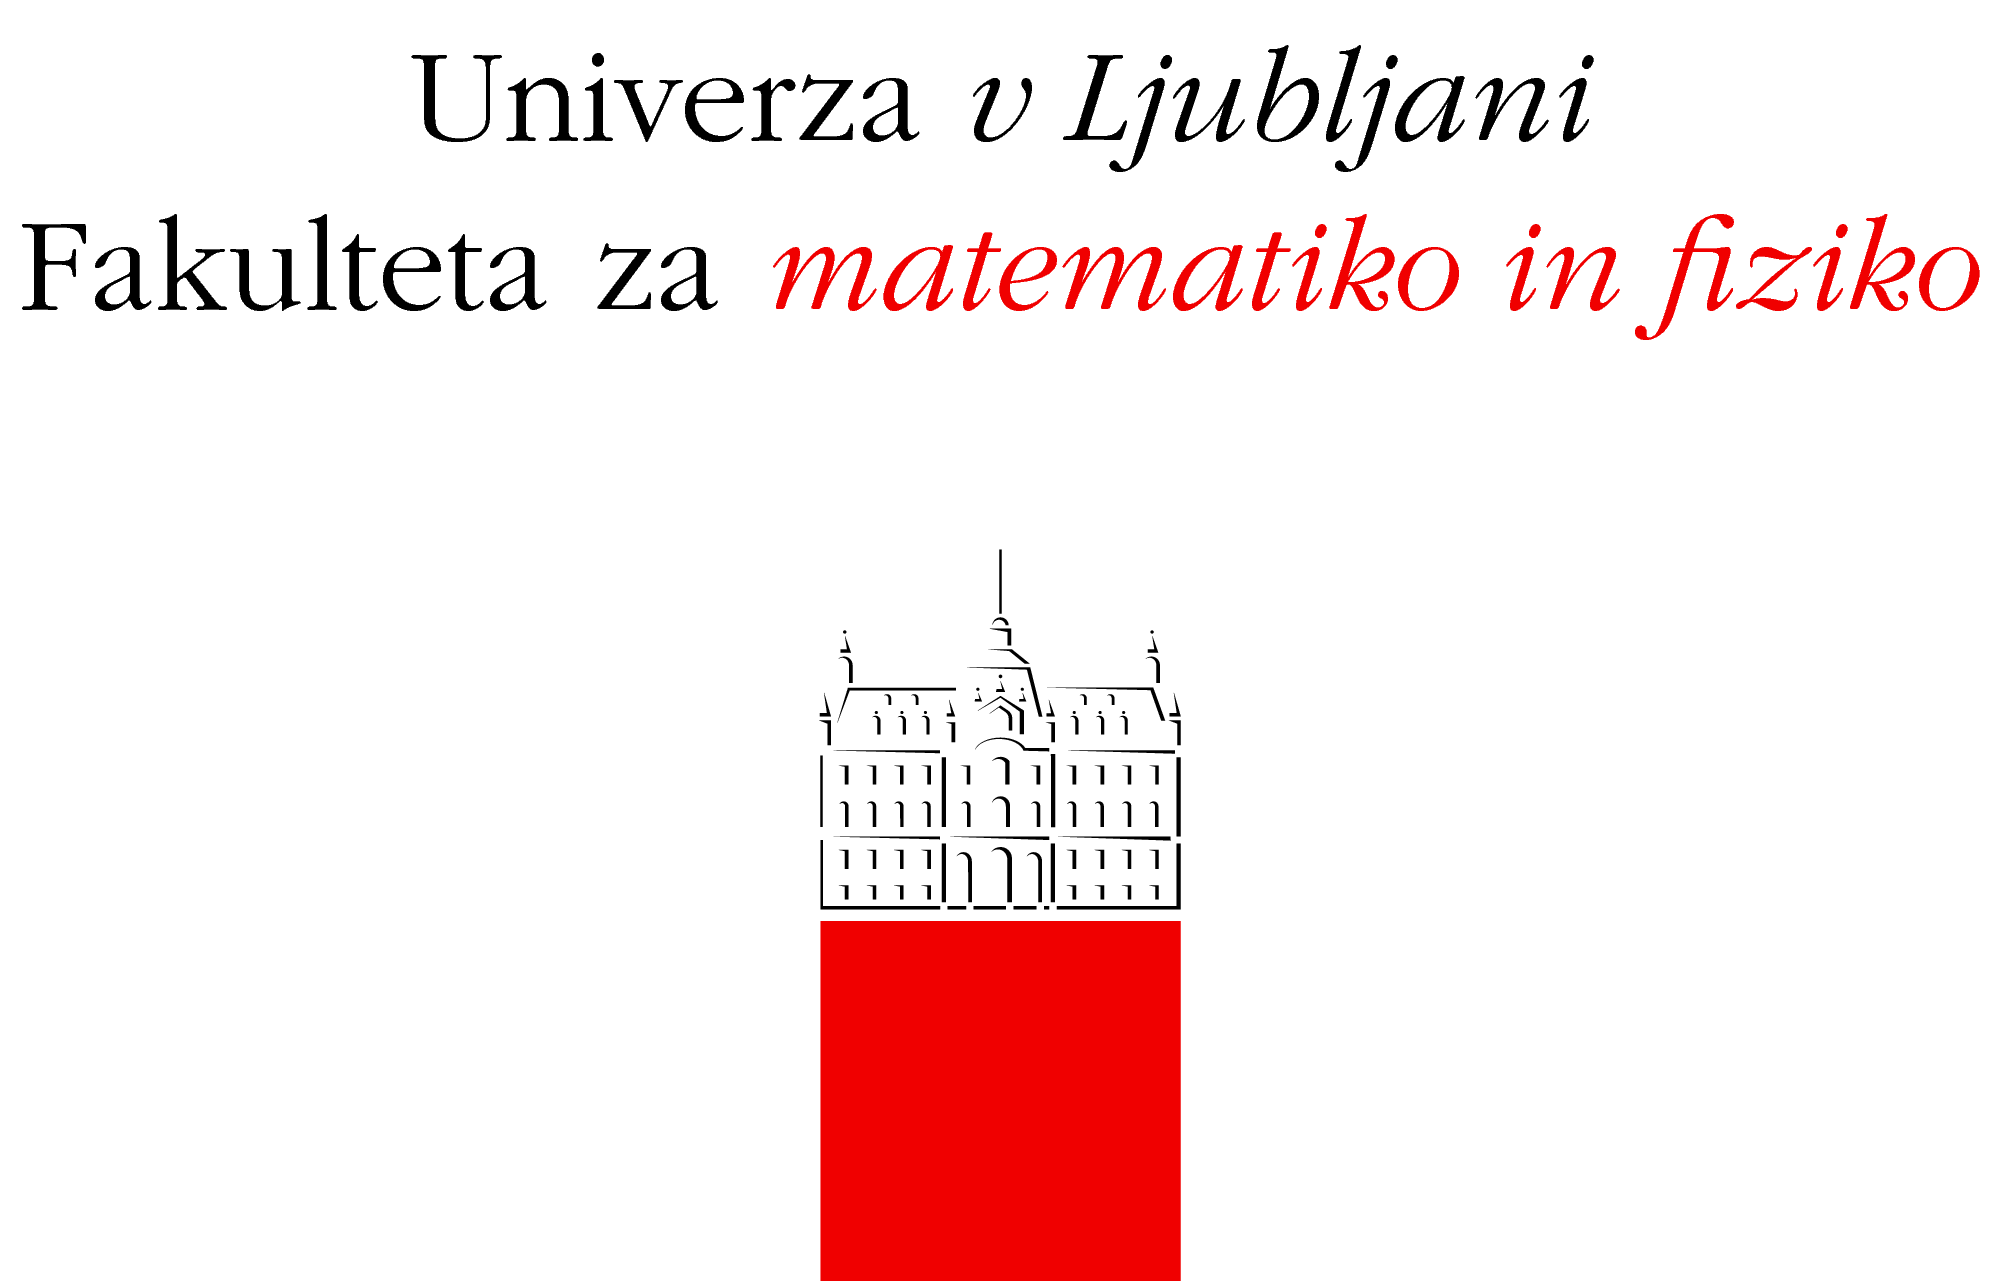
\includegraphics[width=0.45\textwidth]{logo_fmf_uni-lj_sl_veliki.png}\par\vspace{1cm}

	\vspace{1cm}

	\vspace{1.5cm}
	{\huge\bfseries Spectral methods for initial value problem PDE\par}
	\vspace{2cm}
	{\Large Miha Pompe 28191072\par}
	\vfill

	\vfill

% Bottom of the page
	{\large December 2021\par}
\end{titlepage}
% \maketitle
\thispagestyle{empty}
\clearpage
\pagenumbering{arabic}
\newpage


\section{Introduction}
There exist two vast classes of solving initial values problems for partial differential equations. Difference methods use finite differences to approximate time and space derivatives. Thus we convert solving PDEs to solving algebraic equations or systems of equations for the values of the functions. With this exercise we will be focusing on spectral methods, where the solution is expressed using a set of functions and then the coefficients of expansion change with time. We will use two sets of functions: trigonometric (Fourier method) and cubic B-splines (spline method).

In this exercise we will be solving one dimensional diffusion equation for a temperature field ($T(x,t)$) in homogeneous plate of width $a$, without heat sources:

\begin{equation*}
  \frac{\partial T}{\partial t} = D\frac{\partial T}{\partial x} \>, \qquad 0\le x \le a \>, \qquad D={\lambda\over \rho c} \>.
\end{equation*}

\subsection{Fourier method}
The temperature at $x$ and $t$ can be expressed using a Fourier series:
\begin{equation*}
  T(x,t) \simeq \sum_{k=0}^{N-1} \widetilde{T}_k(t)
  e^{-2\pi\mathrm{i} f_k x} \>,
\end{equation*}
where $f_k = k/a$. If we insert the series into the diffusion equation we can solve for $\widetilde{T}_k(t)$ and get:
\begin{equation*}
  T(x,t) \simeq \sum_{k=0}^{N-1} c_k e^{-4\pi^2Df_k^2t}
  e^{-2\pi\mathrm{i} f_k x} \>,
\end{equation*}
At $t=0$, $T(x,0) = x_0(x)$, therefore we can get out the coefficients $c_k$ by performing a Fourier transform on the initial value. 

Afterwards we perform the inverse Fourier transformation to get the solution.

\subsection{B-splines method}
Instead of using trigonometric functions we can use cubic functions to approximate our solution. 
\begin{equation*}
  T(x,t) = \sum_{k=-1}^{N+1} c_k(t) B_k(x) \>,
\end{equation*}
B-spline ($B_k(x)$) is a combination (spline) of cubic functions. Instead of using the Fourier transform we have to solve this problem algebraically. By inserting the equation above into the diffusion equation we can convert this problem into solving a matrix system
\begin{equation*}
  {\bi A}\frac{d\vec{c}}{dt} = {\bi B}\vec{c} \>,
\end{equation*}
where
\begin{equation*}
  {\bi A} = \left[
\begin{array}{ccccccc}
4 & 1 \cr
1 & 4 & 1 \cr
  & 1 & 4 & 1 \cr
  &   &   & \vdots \cr
  &   &   & 1 & 4 & 1 & \cr
  &   &   &   & 1 & 4 & 1 \cr
  &   &   &   &   & 1 & 4
\end{array}
\right] \>, \qquad
{\bi B} = {6D\over{\Delta x}^2} \left[
\begin{array}{rrrrrrr}
-2 & 1 \cr
1 & -2 & 1 \cr
  & 1 & -2 & 1 \cr
  &   &   & \vdots \cr
  &   &   & 1 & -2 & 1 & \cr
  &   &   &   & 1 & -2 & 1 \cr
  &   &   &   &   & 1 & -2
\end{array}
\right]
\end{equation*}
To solve this system we will use a stable implicit method:
\begin{equation*}
  \left( { A} - \frac{\Delta t}{2}{ B}\right)\vec{c}^{\>n+1} \>
  = \left( { A} + \frac{\Delta t}{2}{ B}\right)\vec{c}^{\>n} \>
\end{equation*}
where $T(x_j,0) = x_0(x_j)$ and ${\bi A}\vec{c}^{\>0} = \vec{f}$.

\section{Analysis}

The boundary conditions are divided into periodic and Dirichlet. Periodic conditions are $T(0,t) = T(a, t)$, which can be interpreted as an isolated rod, which is not losing any heat. Homogeneous Dirichlet boundary conditions are $T(0,t) = T(a, t) = 0$, which means we are removing heat from the system by keeping the edges at a constant temperature. The initial condition is a Gaussian distribution of temperature, centered at $a/2$.

Figure 1a shows the solution for periodic conditions using the Fourier method. We can observe the exponential decline of peak temperature over time, which is expected for diffusion equation. With time the edge values start to rise, as the heat evenly distributes across the object.

A similar exponential decline is also seen for Dirichlet boundary conditions (Figure 2c, 2d), the only difference being that the entire distribution approaches $0$ at $t \rightarrow \infty$. The solutions produced using Fourier method (Figure 2c) and spline method (Figure 2d) are very similar. The absolute difference between the two is presented in Figure 2b and we can see that the maximum error decreases with time. One thing to note is that the error heavily relies on the number of steps ($N$), in this example $N = 300$.

\begin{figure}[hbtp]
  \begin{subfigure}{0.5\textwidth}
  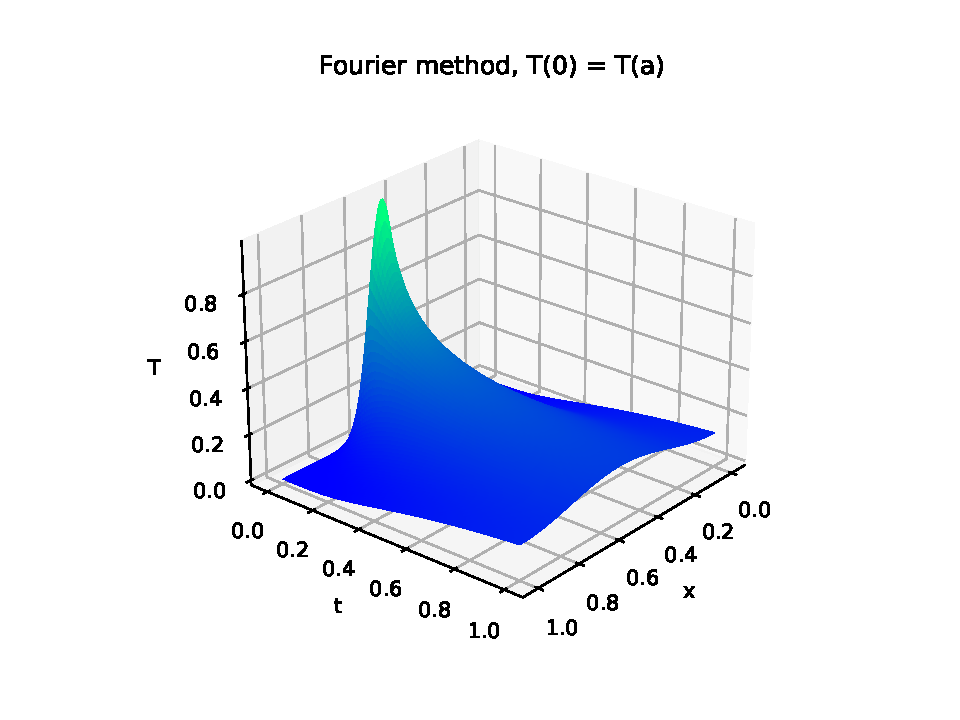
\includegraphics[width=\linewidth]{graphs/1_exercise/fourier_gauss.pdf}
  \caption{Periodic boundary conditions using Fourier method} \label{fig:a}
  \end{subfigure}
  \hspace*{\fill}
  \begin{subfigure}{0.5\textwidth}
  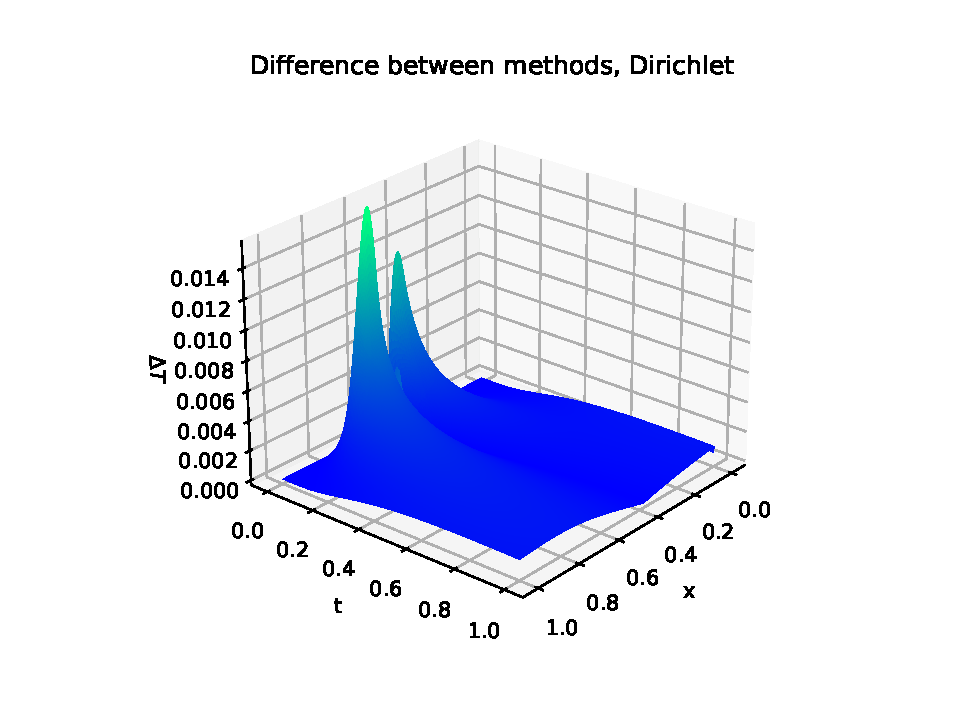
\includegraphics[width=\linewidth]{graphs/1_exercise/difference_gauss.pdf}
  \caption{The absolute difference between Fourier and spline method} \label{fig:b}
  \end{subfigure}
  \medskip
  \begin{subfigure}{0.5\textwidth}
  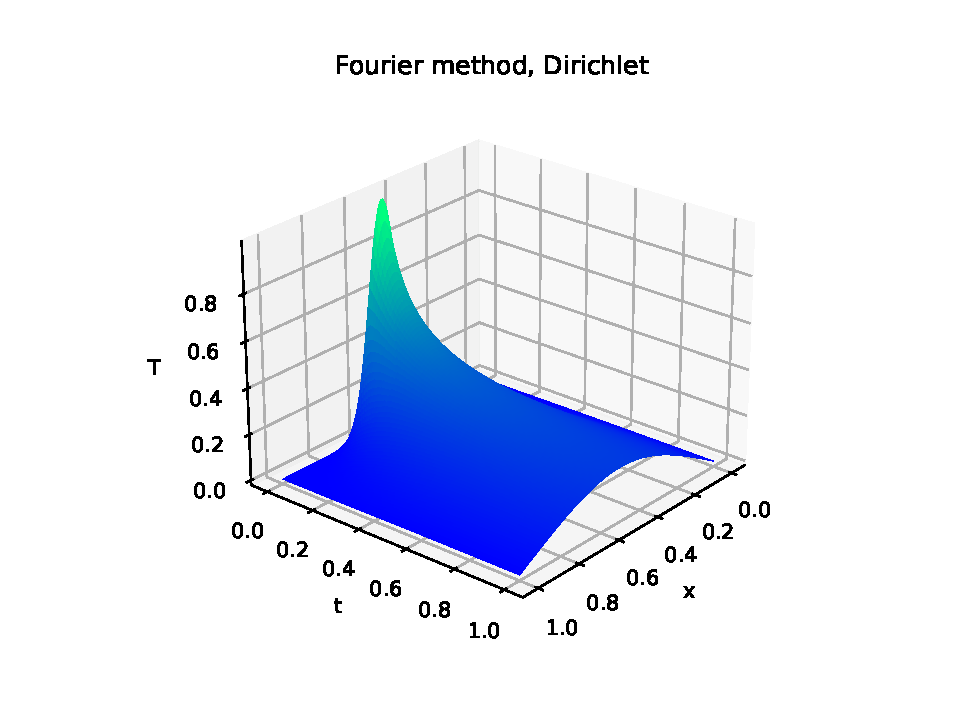
\includegraphics[width=\linewidth]{graphs/1_exercise/fourier_gauss_dirichlet.pdf}
  \caption{Dirichlet boundary conditions using Fourier method} \label{fig:c}
  \end{subfigure}
  \hspace*{\fill}
  \begin{subfigure}{0.5\textwidth}
  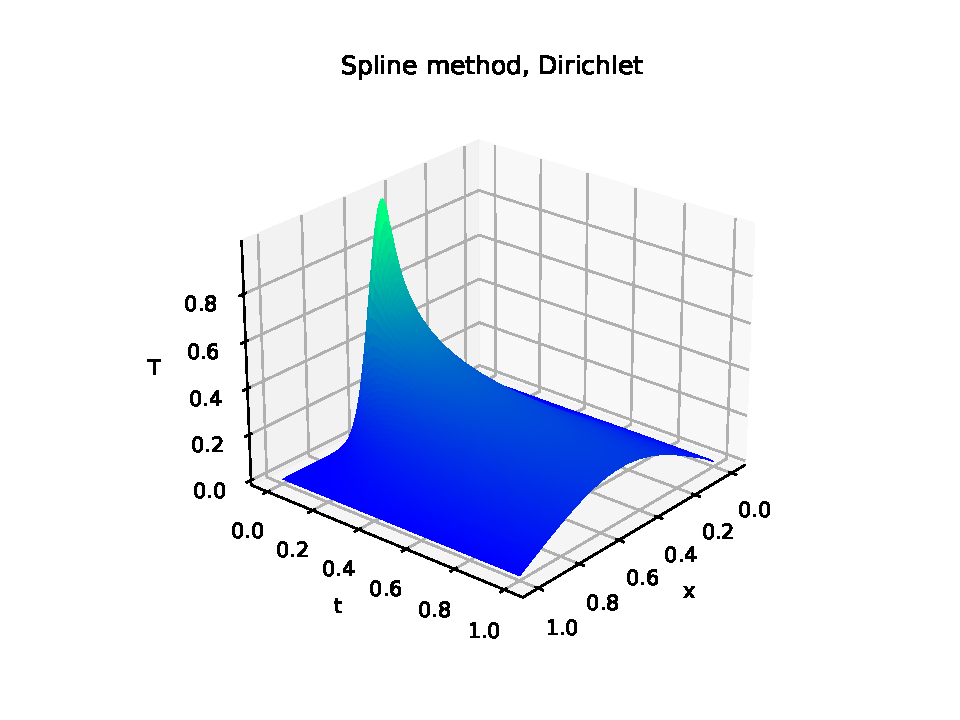
\includegraphics[width=\linewidth]{graphs/1_exercise/spline_gauss_dirichlet.pdf}
  \caption{Dirichlet boundary conditions using spline method} \label{fig:d}
  \end{subfigure} 
  \caption{Diffusion equation solutions with Gaussian initial function} \label{fig:1}
\end{figure} 

For a better visualization of previous statements let's look at Figure 2a and 2b. The former shows the temperature at the midpoint ($T(a/2, t)$). The value goes to zero with Dirichlet conditions and settles at a constant value with periodic conditions. The area under the graph is proportional to the total amount of energy stored in the system. Figure 2b shows that the energy doesn't change with periodic conditions and goes to zero with Dirichlet conditions.

\begin{figure}[hbtp]
  \begin{subfigure}{0.5\textwidth}
  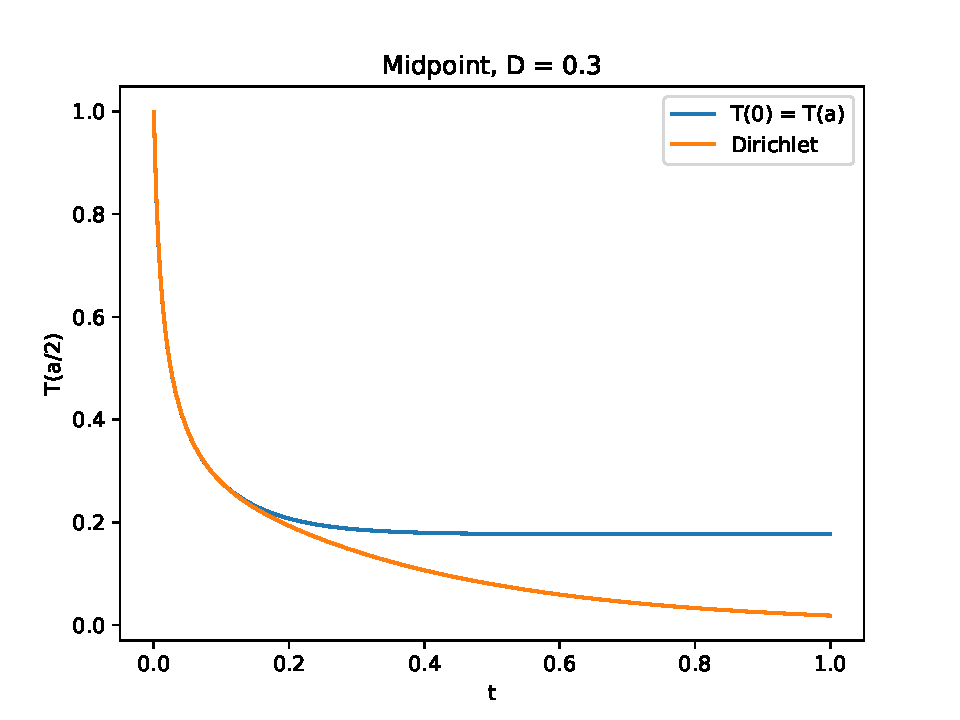
\includegraphics[width=\linewidth]{graphs/2_analysis/energy.pdf}
  \caption{The midpoint value over time} \label{fig:c}
  \end{subfigure}
  \hspace*{\fill}
  \begin{subfigure}{0.5\textwidth}
  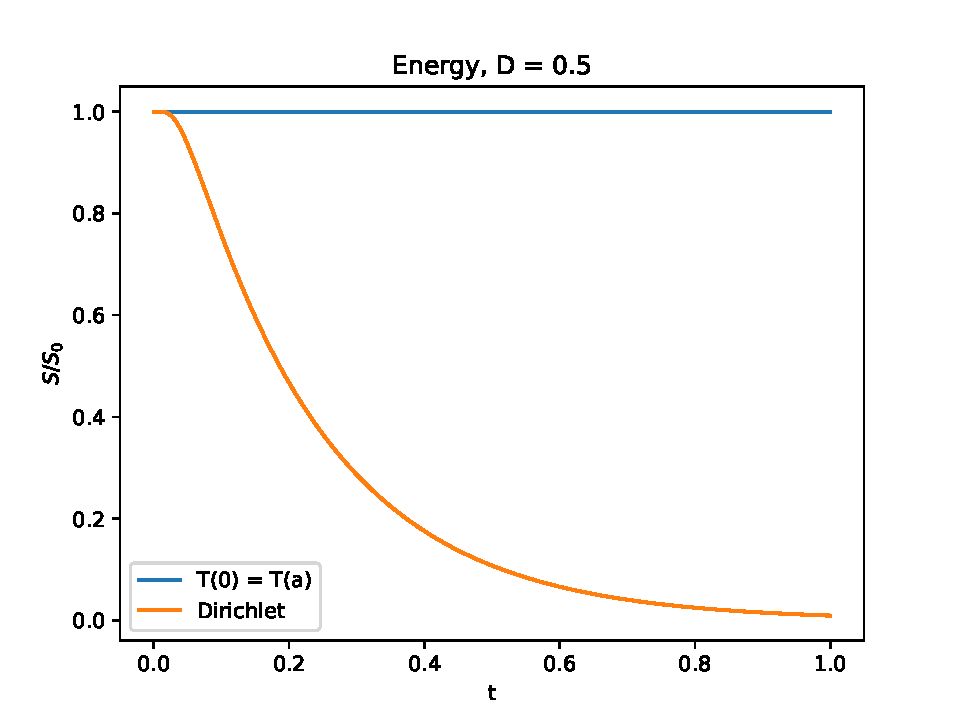
\includegraphics[width=\linewidth]{graphs/2_analysis/energy2.pdf}
  \caption{The total energy of the system over time} \label{fig:d}
  \end{subfigure} 
  \medskip
  \begin{subfigure}{0.5\textwidth}
  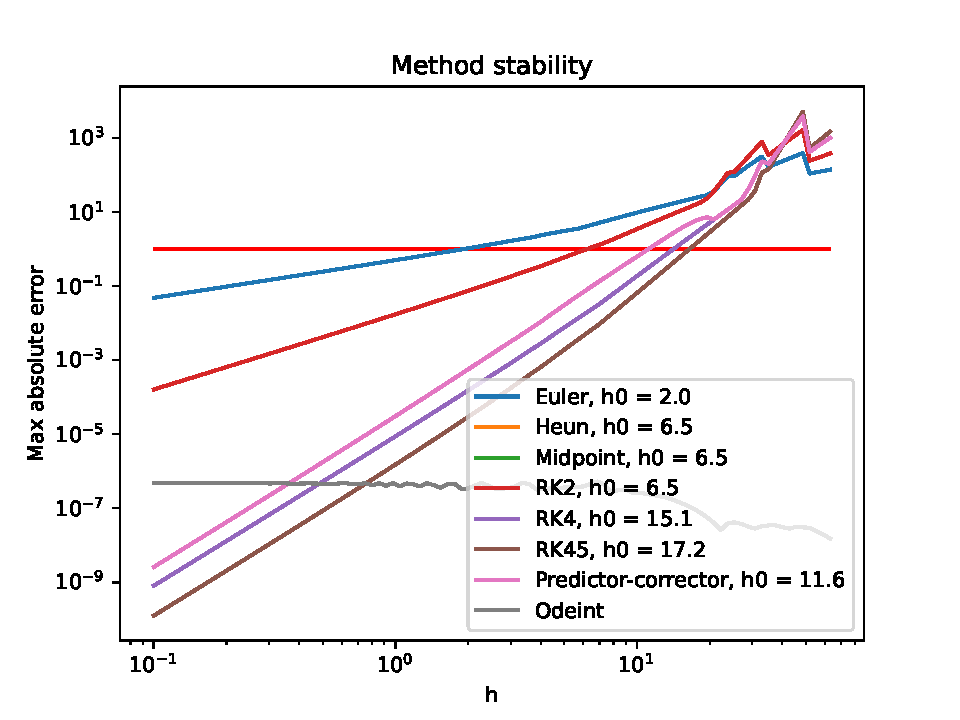
\includegraphics[width=\linewidth]{graphs/2_analysis/stability.pdf}
  \caption{Stability of methods with respect to $N$} \label{fig:a}
  \end{subfigure}
  \hspace*{\fill}
  \begin{subfigure}{0.5\textwidth}
  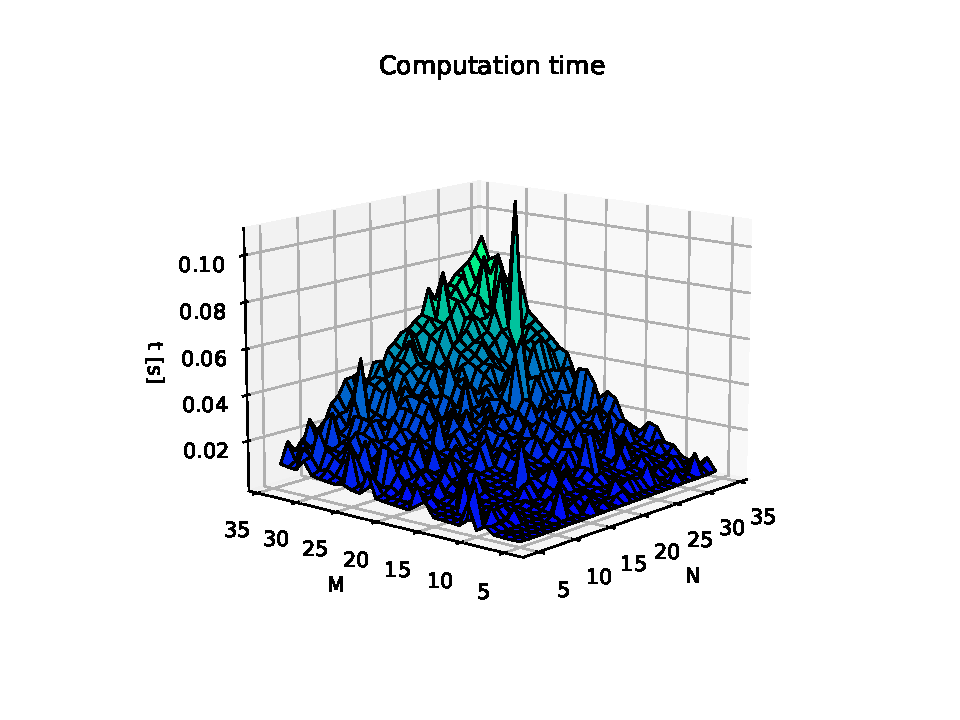
\includegraphics[width=\linewidth]{graphs/2_analysis/time.pdf}
  \caption{Computation time, fit $t = N^n$} \label{fig:b}
  \end{subfigure}
  \caption{Analysis of numerical methods} \label{fig:1}
\end{figure}

The number of point in the time and space interval is $N$ ($N = a/h_x = t_{max}/h_t$). The performance of both numerical methods highly depends on this parameter. Figure 2c shows the maximum values of $T$ at discrete times for different $N$, which can be interpreted as stability. For an ideal method all of these lines should be straight. The biggest deviations can be seen with lower values of $N$ where we only have a small number of functions to approximate our solution with. The Fourier method is more unstable compared to spline methods. In general as $N > 150$ both methods become stable. This result is dependent on the initial conditions.

\begin{figure}[hbtp]
  \begin{subfigure}{0.5\textwidth}
  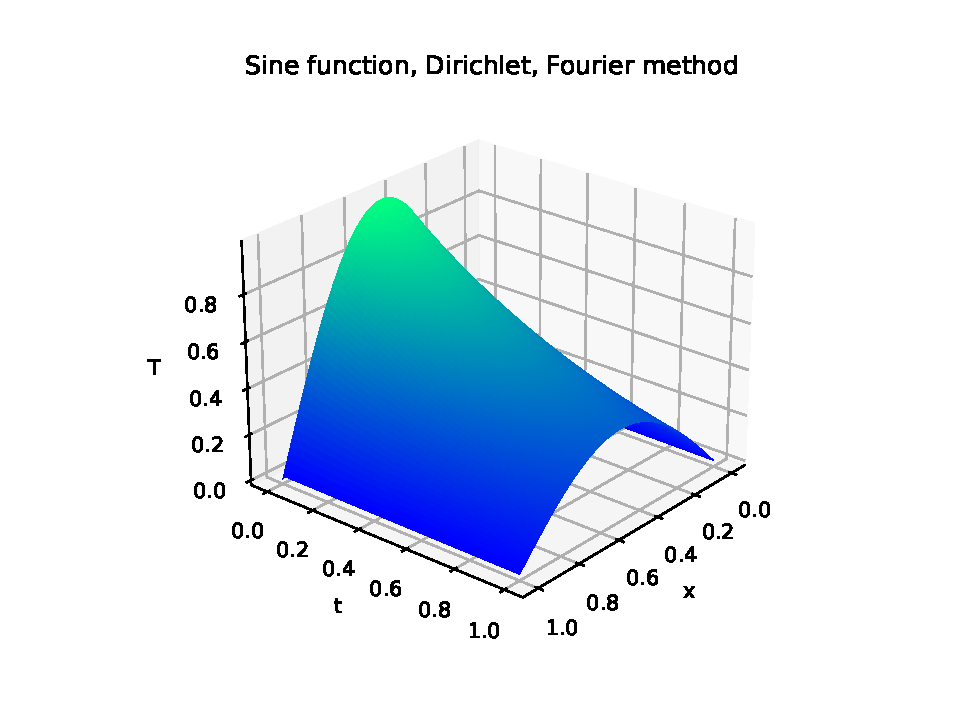
\includegraphics[width=\linewidth]{graphs/3_dodatna/sine.pdf}
  \caption{Sine function, $\omega = 1$} \label{fig:a}
  \end{subfigure}
  \hspace*{\fill}
  \begin{subfigure}{0.5\textwidth}
  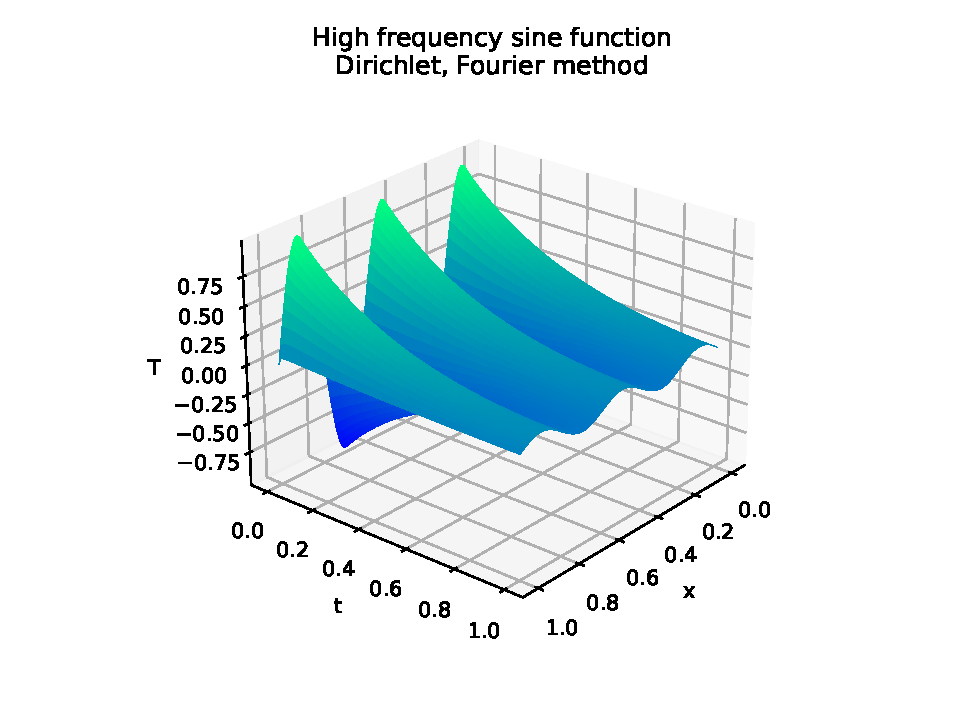
\includegraphics[width=\linewidth]{graphs/3_dodatna/sine_high.pdf}
  \caption{Sine function, $\omega = 5$} \label{fig:b}
  \end{subfigure}
  \medskip
  \begin{subfigure}{0.5\textwidth}
  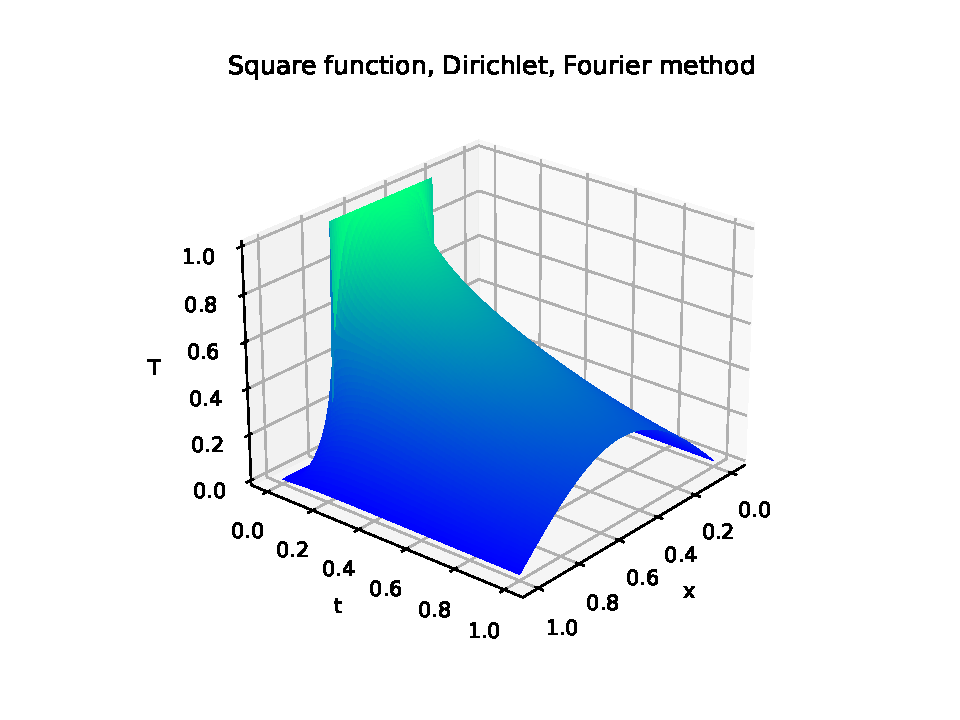
\includegraphics[width=\linewidth]{graphs/3_dodatna/square.pdf}
  \caption{Square function} \label{fig:c}
  \end{subfigure}
  \hspace*{\fill}
  \begin{subfigure}{0.5\textwidth}
  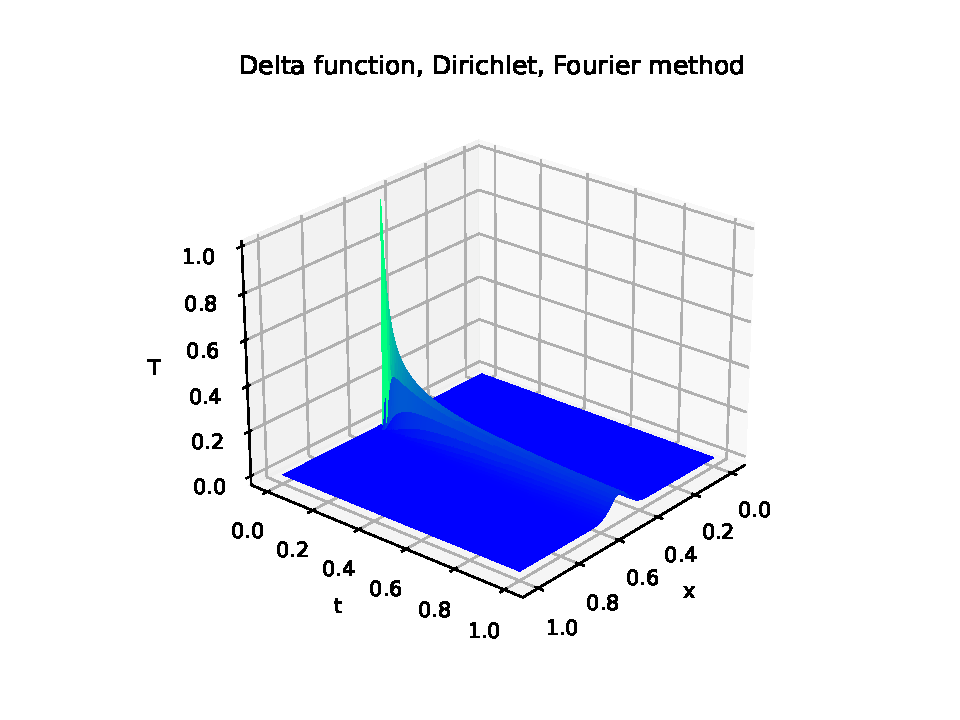
\includegraphics[width=\linewidth]{graphs/3_dodatna/delta.pdf}
  \caption{Delta function} \label{fig:d}
  \end{subfigure} 
  \caption{Solutions to different initial functions computed using Fourier method for Dirichlet boundary conditions.} \label{fig:1}
\end{figure}

The second factor we will look at is computation time of both methods. Figure 2d shows that complexity of the Fourier method is $\mathcal{O}(N)$ and the spline method in $\mathcal{O}(n^3)$. The implemented Fourier method uses fast Fourier transform with time complexity of $\mathcal{O}(nlogn)$. Other computation steps don't contribute a lot to the overall complexity. The most time consuming step of the spline method is computing an inverse and solving a system of equations (size $N \times N$), both of these methods are $\mathcal{O}(N^3)$. 

The last two analysis steps were performed using Dirichlet boundary conditions.

Let's now analyse different initial functions. Figure 3a and 3b shows how an initial sine distribution changes with time. With respect to time the function drops exponentially, but with respect to $x$ the function remains a sine wave. Separation of variables gives us the same result. The difference between high and low frequency oscillations changes how quickly we reach equilibrium, which is a consequence of derivatives having higher values.

Taking this to the extreme we can examine a square (Figure 3c) and a delta function (Figure 3d). The sharp corners get rounded very quickly. Afterwards the progression behaves similar to Gaussian or sine examples.

\end{document}

